% tex file for convolution
\subsubsection{Convolution}
\par \indent Our study is structured around event-related neurological 
stimulus, not block stimulus as was discussed in the in-class example. We 
predicted the hemoglobin response (HR) related to this type of neurological 
stimulus. 

There were multiple ways in which we approached the problem of trying to 
better replicate the predicted response function defined by:

\begin{equation} \label{eq:convolve}
r(t)= \sum_{i=1}^n \psi_{i} \phi_{i}(t-t_i)
\end{equation}

where $\psi$ is the amplitude of the response stimulus (always $1$ in our 
case), and $\phi_{i}$ is the hemodynamic response started at the $i$th 
stimulation ($t_i$).

The five approaches we attempted can be divided into 3 subcategories: 
\textbf{(1)} a strict replication of \ref{eq:convolve}; \textbf{(2)} a similar 
function as \textbf{(1)} that utilizes matrix multiplication; and \textbf{(3)} a 
function that splits the intervals between each scan (2 seconds) into a certain 
number of even slices, then puts the stimulus into the closed split, using 
\texttt{np.convolve} on this stimulus and a detailed hrf function, and then 
reducing the output back into the 2-second time intervals. Detailed exploration 
of this matter can be found in the appendix.

We compared these methods based on accuracy and speed. [Figure 
\ref{fig:convolution}] displaces accuracy comparison, and the table in 
[Table~\ref{tab:convolution}] show the accuracy based off of \texttt{ipython}'s 
\texttt{timeit} function.



\begin{figure}[ht]
\centering
	\begin{minipage}[b]{0.45\linewidth}
		\centering
		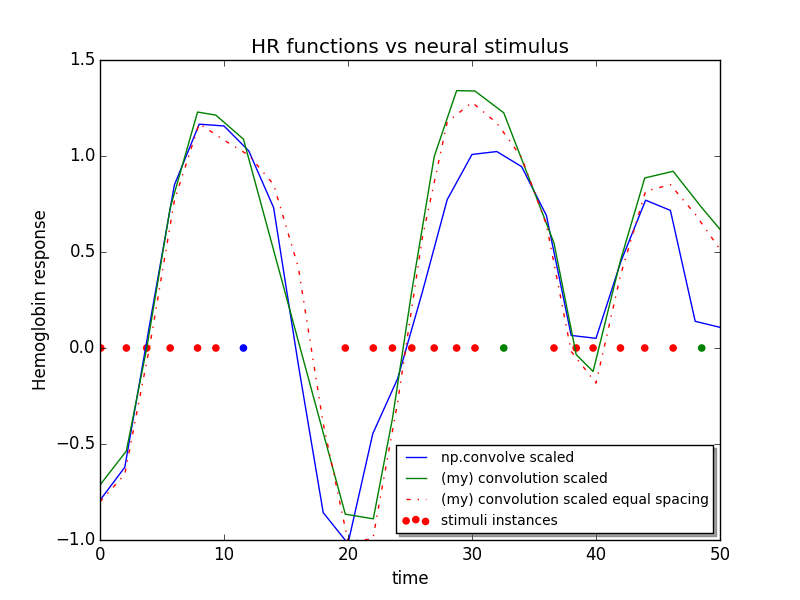
\includegraphics[width=.8\linewidth]{images/convolution_vs_neural_stimulus}  
		% needs to be from the event_related_HRF_script2.py 
		\caption{\scriptsize{Different convolution functions vs. the Neural stimulus}}
		\label{fig:convolution}

	\end{minipage}
\quad
	\begin{minipage}[b]{0.45\linewidth}
		\centering
		\begin{tabular}{|l | c|}
		\hline
		name in graph       & Speed per loop \\
		\hline
		np naive approach & 14.4 $\mu$s  \\
		user 2     		    & 972 ms  \\
		user 3     		    & 1.15 s    \\
		user 4 (15 cuts)      & 98.3 ms \\
		user 4 (30 cuts)      & 185 ms  \\
		user 5     	 	    & 110 ms   \\
		\hline
		\end{tabular}
		\vspace{5mm}
		\label{tab:convolution}
		\captionof{table}{\scriptsize{Speed to create HRF predictions for Subject 001, 
		all conditions}}
	\end{minipage}
\end{figure}

The ``np naive approach'' run has the worst approximation and isn't even 
theoretically correct. As was stated above, this was the large motivating factor 
behind the rest of the convolution analysis. The ``user 2'' and ``user 3'' runs fall 
under subcategory \textbf{(1)}. The ``user 2'' was the first approach to
matches the theory, but matches the stimulation times and not the scan times.
The ``user 3'' is the most theoretically sound model (and is our standard for 
accuracy). The ``user 5'' falls under subcategory \textbf{(2)}, ``User 5''  is our 
matrix version of the theory, and has the same accuracy as ``user 3''. The 
``user 4'' model fall under subcategory \textbf{(3)}, the methods that use the 
grid cut usage of \texttt{np.convolve} with notations for the number of slices 
between each scan.

\subsubsection{Time Correction}

The fMRI machine scans each voxel at a slightly different time. In our case, 
the lowest horizontal slice was scanned first, with the later scans moving 
progressively toward the top of the brain. So, there is an observable time drift 
that needs be accounted for. We did so by shifting the times of stimulus 
``backwards'' for voxels scanned later to directly "correct" for the delay of 
the scan (assuming that each layer of the scan took 2/34 of a second).

\subsubsection{Multiple Conditions}

At the beginning of our analysis we tried to see if there was an advantage to 
separating our 3 conditions and creating separate predicted hemodyamic reposes 
for each to allow for different amplitudes for each type of condition. We did 
not observe a large difference in the $\hat{\beta}$ values we got, so we did not 
continue with this exploration. It is quiet possible that with the new 
approaches we've applied, differentiating the conditions for the stimulus might 
see gains in interpretability.


